% 2007 年安徽卷文科第 7 题：定义在 [0,2] 上的折线图象，x=0 与 x=2 处为 0，
%   x=1 处为 3/2，两侧各为直线段。
% 来源 PDF：gaokaomath-src/普通高考/2007/2007安徽文.pdf
% SHA-256：dc00a80c0b71b6d66708ceef533f06f1d54c35ac1e64b122d72e2df9779b2450
% 原页：2007安徽文.pdf 第 1 页（A3 三栏）第 1 栏，书页码 349，图在第 7 题题干下方。
% 重绘依据：按 (0,0)-(1,3/2)-(2,0) 作折线，x 轴画到 2 右侧并标箭头，y 轴标到 3/2 上方；
%   在 x=1 处画虚线竖线到曲线并标 y 轴刻度 3/2；x 轴刻度 1、2 与原点 O 标注。
\begin{tikzpicture}[scale=1.35, semithick,
  every node/.style={inner sep=1.5pt}]
  % 坐标轴
  \draw[->] (-0.3,0) -- (2.55,0) node[anchor=west] {$x$};
  \draw[->] (0,-0.25) -- (0,1.85) node[anchor=south] {$y$};
  % 折线
  \draw (0,0) -- (1,1.5) -- (2,0);
  % 顶点虚线
  \draw[dashed] (1,0) -- (1,1.5);
  % 刻度
  \draw (1,0.05) -- (1,-0.05);
  \draw (2,0.05) -- (2,-0.05);
  \draw (0.05,1.5) -- (-0.05,1.5);
  % 标注
  \node[anchor=north east] at ([xshift=-2pt,yshift=-3pt]0,0) {$O$};
  \node[anchor=north] at ([yshift=-3pt]1,0) {$1$};
  \node[anchor=north] at ([yshift=-3pt]2,0) {$2$};
  \node[anchor=east] at ([xshift=-3pt]0,1.5) {$\dfrac32$};
\end{tikzpicture}
